
\section{Matrix completion and skewed distribution of ratings} \label{ch:matcomp:hypoexp}
As described in Section~\ref{ch:related}, the matrix completion-based methods
can accurately recover the underlying low-rank model of a given low-rank matrix
provided entries are observed uniformly at random from the matrix.
However, the ratings in the user-item rating matrix in real-world datasets
do not represent a random sample of entries because some items receive few
ratings and some users have rated few items, thus leading to a skewed distribution of 
ratings in the matrix.
In the following sections, we will try to answer the question how does the skewed 
distribution of ratings in real datasets affects the accuracy and the ranking
performance of the matrix completion-based methods. 
Furthermore, we will try to understand how does the performance of matrix
completion-based methods changes with the number of ratings an item have.

%=========================================================================
\subsection{Experiment design} \label{sec:ch:matcomp:expdesign}
In order to study how the skewed distribution of ratings in real datasets
affects the ability of matrix completion to accurately complete the matrix (i.e.,
predict the missing entries) we performed a series of experiments using synthetically
generated low-rank rating matrices. 
%
In order to generate a rating matrix $R\in \mathbb{R}^{n\times m}$ of rank $k$ we
followed the following protocol. We started by generating two matrices
$A\in\mathbb{R}^{n\times k}$ and $B\in\mathbb{R}^{m\times k}$ whose values are
uniformly distributed at random in $[0, 1]$. We then computed the singular value
decomposition of these matrices to obtain $A=U_A\Sigma_A V_A^T$ and $B=U_B\Sigma_B
V_B^T$. We then let $P=\alpha U_A$ and $Q=\alpha U_B$ and $R = PQ^T$. Thus, the final
rank $k$ matrix $R$ is obtained as the product of two randomly generated rank $k$
matrices whose columns are orthogonal. Note that the parameter $\alpha$ was
determined empirically in order to produce ratings in the range of $[-10, 10]$.

We used the above approach to generate full rating matrices whose dimensions are
those of the four real-world datasets shown in Table~\ref{table:ch:matcomp:datasets_table}. For
each of these matrices we used two approaches to select the subset of their entries
that will be given as input to the matrix completion algorithm. The first approach
selects the entries that correspond to the actual user-item pairs that are present in
the corresponding dataset, whereas the second approach selects the entries uniformly
at random from the entire matrix. The number of entries that are selected by both
approaches is the same and is the number of non-zeros in the actual dataset (shown in
Table~\ref{table:ch:matcomp:datasets_table}). 

The advantages of working with this type of synthetically generated datasets are
two-fold. First, by construction we can ensure that the underlying matrix is of known
(low) rank. Second, since we know the values of the full matrix, we can easily
measure how accurately the low-rank models estimated using matrix completion can
complete the entire matrix. 


In order to estimate the low-rank factor matrices from the observed entries
(Equation~\ref{mf_obj}) we used Stochastic Gradient Descent~\cite{bottou2010large} and
initialized the factor matrices with the singular vectors of the rating matrix by
assuming that the missing entries were rated as 0, which is shown to converge closer
to global minimum~\cite{JainSanghavi13}. 
%
For each dataset we generated five different sets of matrices using different random
seeds and we performed a series of experiments using synthetically generated low-rank
matrices of rank 5, 10, and 20. For each rank, we report the average of performance
metrics in each set from the estimated low-rank models over all the synthetic
matrices.

To simplify the discussion, we will refer to the set of matrices derived from the
actual sparsity structure of the real datasets as \emph{SYN-REAL} and from the
randomly sampled entries as \emph{SYN-RAND}. In addition we will refer to the values
of the synthetically generated rating matrices as \emph{ground-truth} in order
to differentiate them from the values predicted as part of matrix completion.

\begin{table}[bt]\small
  \centering
  \caption{Datasets used in experiments} \label{table:ch:matcomp:datasets_table}
  \begin{threeparttable}
    \begin{tabular}{
        @{\hspace{2pt}}l@{\hspace{3pt}}|
        @{\hspace{2pt}}r@{\hspace{3pt}}
        @{\hspace{2pt}}r@{\hspace{3pt}}
        @{\hspace{2pt}}r@{\hspace{3pt}}
        @{\hspace{2pt}}r@{\hspace{3pt}}
        @{\hspace{2pt}}r@{\hspace{3pt}}
        @{\hspace{2pt}}r@{\hspace{3pt}}
        @{\hspace{2pt}}r@{\hspace{3pt}}
        @{\hspace{2pt}}r@{\hspace{3pt}}
      }
      %\toprule
      \hline
      \textbf{Dataset} & \textbf{users} & \textbf{items}  & \textbf{ratings} &
           \textbf{$\mu_u$}\tnote{a} &
         \textbf{$\sigma_u$}\tnote{b} &
            \textbf{$\mu_i$}\tnote{c} & \textbf{$\sigma_i$}\tnote{d} &
            \multicolumn{1}{p{0.75cm}}{\centering density \\(\%)\tnote{\textdagger}} \\
            %\textbf{density    (\%)}\tnote{\textdagger} \\
      \hline
      %\BX & 17,219 & 36,546 & 574,127 & 33.34 & 15.70 \\ %& 0.0009\% \\
      \EM (EM) & 61,265 & 1,623 & 2,811,983 & 45.89 & 59.48 & 1732.58 & 3882.55
               & 2.8 \\
    \FLIX (FX) & 147,612 & 48,794 & 8,196,077 & 55.52 & 225.81 & 167.97 & 934.47 & 0.1 \\
      %\MLOM & 6,040 & 3,706 & 1,000,209     \\ %& 165.59 & 269.88 & 0.044\% \\
    \MLTM (ML) & 229,060 & 26,779 & 21,063,128 & 91.95 & 190.53 & 786.55 &
          3269.45 & 0.3 \\
         \NF (NF) & 480,189 & 17,772 & 100,480,507 & 209.252 & 302.33 & 4550.75
                  & 16908.40 & 1.1 \\
      %\YMovies & 7,642 & 11,916 & 221,367   \\ %& 28.96 & 18.57 & 0.002\% \\
      %\YMusic & 100,000 & 50,000 & 11,529,569 \\%& 115.29 & 230.59 & 0.002\% \\
      \hline
    \end{tabular}
    \begin{tablenotes}
      \item[a] The number of average ratings per user in the dataset.
      \item[b] The standard deviation of ratings per user in the dataset.
      \item[c] The number of average ratings per item in the dataset.
      \item[d] The standard deviation of ratings per item in the dataset.
      \item[\textdagger] The percentage of observed ratings in the dataset.
    \end{tablenotes}
  \end{threeparttable}
\end{table}

%========================================================================================%

\subsection{Accuracy of the estimated low-rank models} \label{ch:matcomp:mf_accu}

\begin{table}[bt]
  %\centering
  \caption{RMSE of the estimated low-rank models for different sparsity structures.} 
  \label{table:ch:matcomp:rmse_table}
  \begin{tabular}[t]{lccc}
    \hline
    Dataset
    &\multicolumn{1}{p{0.75cm}}{\centering Rank}
    &\multicolumn{1}{p{1.85cm}}{\centering RMSE for SYN-REAL matrices} 
    &\multicolumn{1}{p{1.85cm}}{\centering RMSE for SYN-RAND matrices} \\
    \hline
    %\multirow{2}{*}{\BX}  & 5 & 1.236   & \underline{0.191} \\ 
    %                      & 10 & \underline{2.014}  & 3.391\\
    %                      & 20 & \underline{2.400}  & 2.850 \\
    %\hline
    \multirow{3}{*}{EM}  & 5 & 0.675 & \underline{0.028} \\
                          & 10 & 1.110 & \underline{0.052}\\
                          & 20 & 1.229 & \underline{0.165} \\
    \hline
    \multirow{2}{*}{FX} & 5 & 1.962 & \underline{0.028}  \\
                           & 10 & 2.225 & \underline{0.053} \\
                           & 20 & 2.425 & \underline{0.167} \\
    \hline
  \end{tabular}
  \hfill
  \begin{tabular}[t]{lccc}
    \hline
    Dataset
    &\multicolumn{1}{p{0.75cm}}{\centering Rank}
    &\multicolumn{1}{p{1.85cm}}{\centering RMSE for SYN-REAL matrices} 
    &\multicolumn{1}{p{1.85cm}}{\centering RMSE for SYN-RAND matrices} \\
    \hline
    %\multirow{2}{*}{\BX}  & 5 & 1.236   & \underline{0.191} \\ 
    %                      & 10 & \underline{2.014}  & 3.391\\
    %                      & 20 & \underline{2.400}  & 2.850 \\
    %\hline
    \multirow{3}{*}{ML} & 5  & 1.377 & \underline{0.024} \\
                           & 10 & 1.222 & \underline{0.039}\\
                           & 20 & 1.872 & \underline{0.074}\\
    \hline
    \multirow{3}{*}{NF}   & 5 & 0.246 & \underline{0.023} \\
                           & 10 & 0.425 & \underline{0.034} \\
                           & 20 & 0.621 & \underline{0.052}\\
    \hline
  \end{tabular}
\end{table}

Table~\ref{table:ch:matcomp:rmse_table} shows the Root Mean Square Error (RMSE) achieved by
the models estimated using both the SYN-REAL and SYN-RAND matrices over the
complete rating matrix.


As can be seen in the table, the RMSE of the low-rank models estimated using the
randomly sampled entries is lower than those estimated using the actual entries.
Additionally, the RMSE increases with the increase in the rank for both sets of
matrices. This is because, as mentioned in Section~\ref{ch:matcomp:intro}, the required number of observed entries to complete
the matrix accurately increases linearly with the rank of the
matrix. 
The RMSE for the SYN-REAL matrices in NF is lower than that of the
others because it has more ratings for both users and items, thus leading to
more accurate estimation of low-rank models.
The higher RMSE in the SYN-REAL matrices compared to that of the SYN-RAND
matrices suggest that the estimated low-rank model fails to recover the missing entries
accurately in the SYN-REAL matrices. This failure can result in
poor predictions for a user on some items and hence impact the recommendations
served to the user.

\begin{figure}[ht]
  %\centering
  %\hspace*{-1cm}
  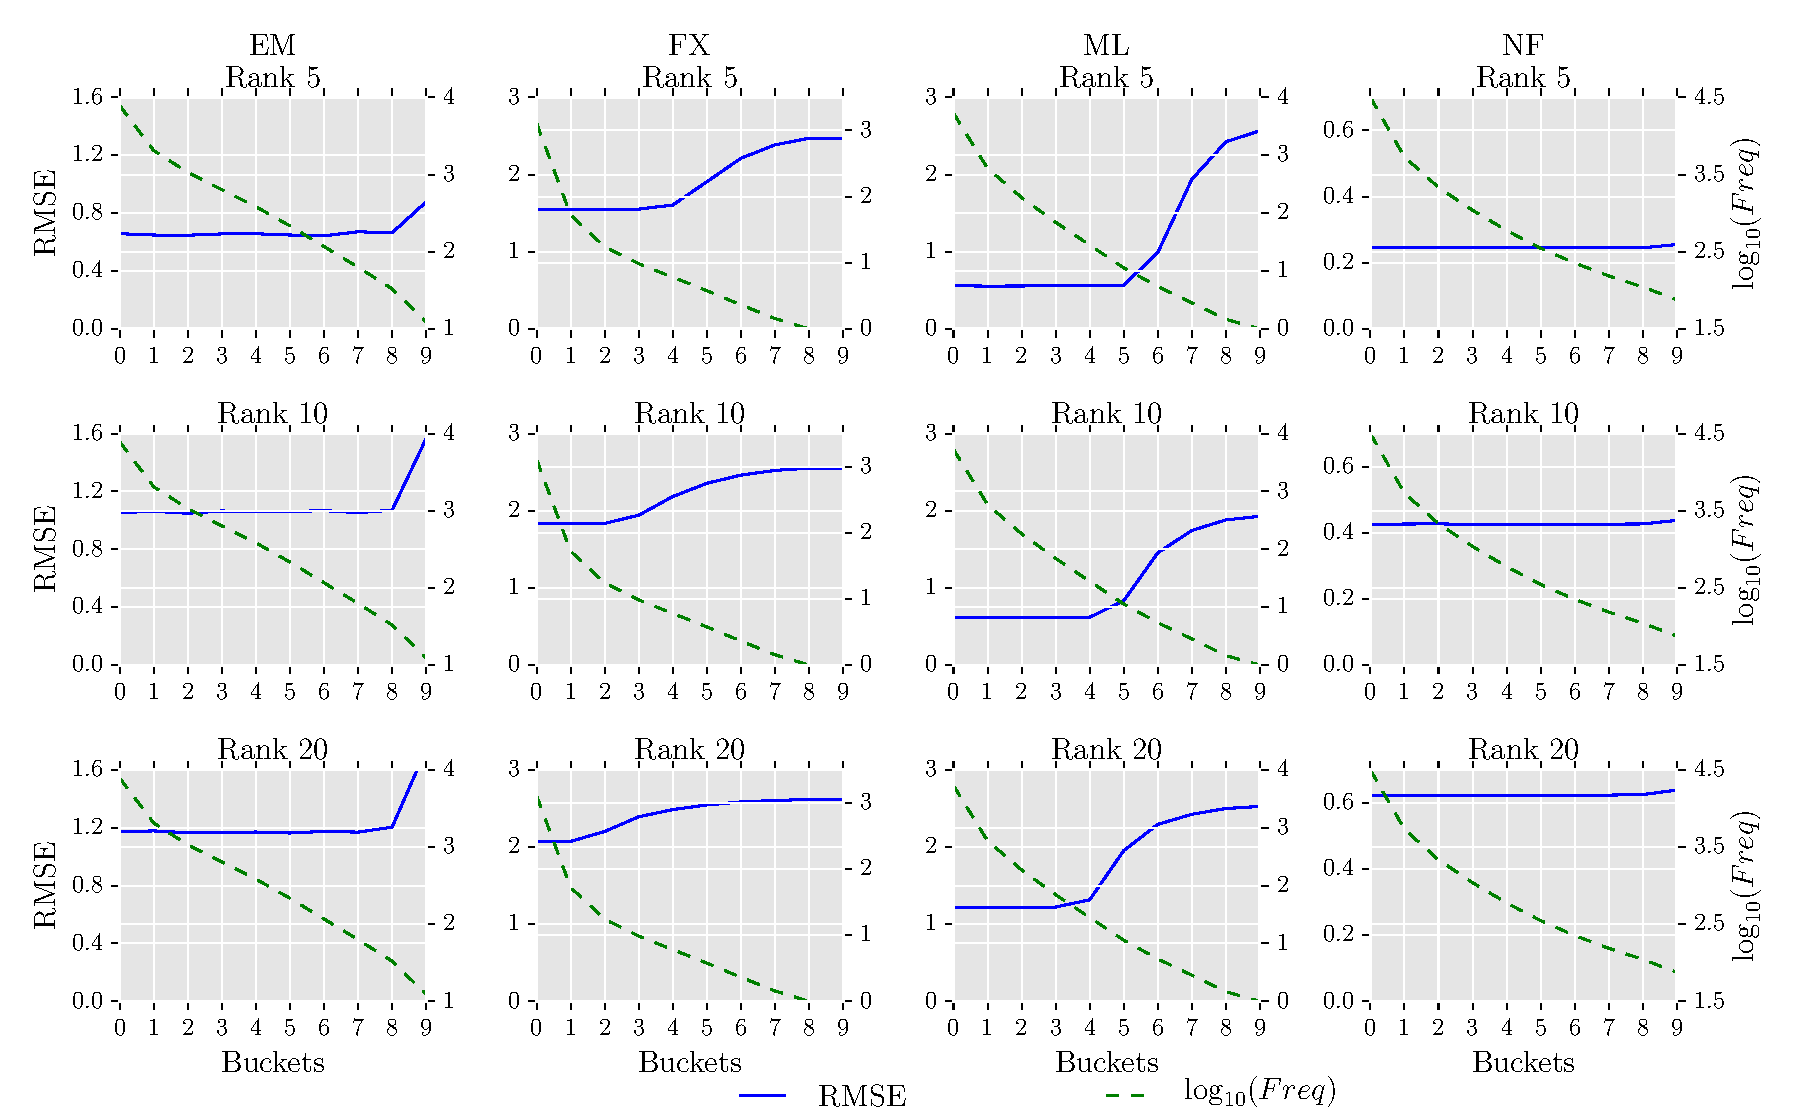
\includegraphics[scale=0.49]{figures/freq_rmsebuckets}
  \caption{RMSE of the predicted ratings as the frequency of the items decreases.}
  \label{fig:freqRMSEbuck}
\end{figure}

\begin{figure*}[hbt]
  %\hspace*{-.75cm}
  %\centering
  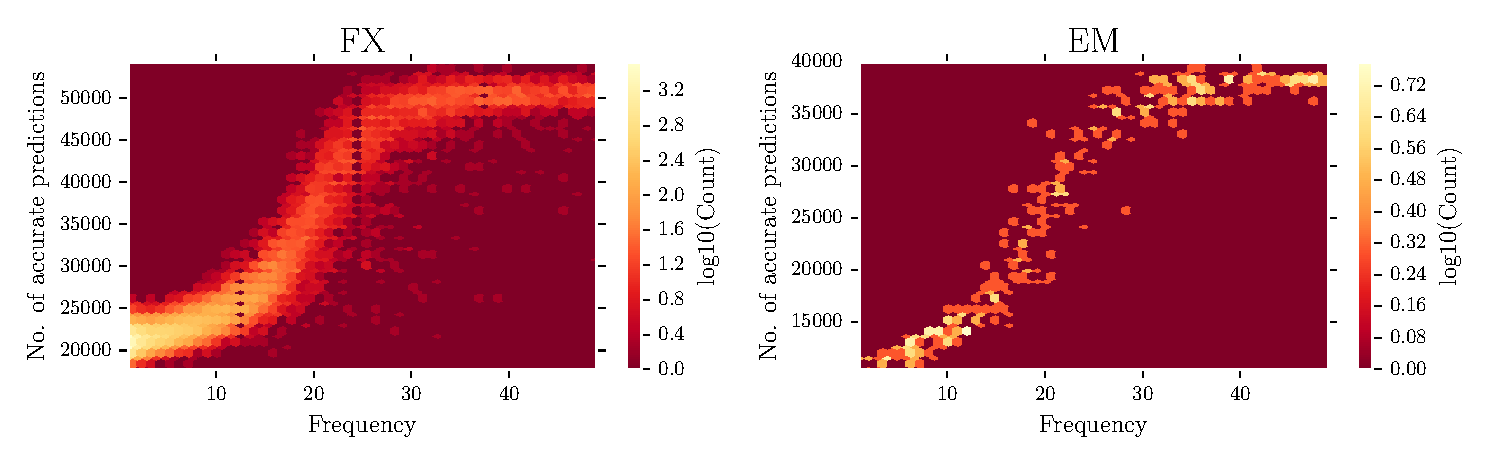
\includegraphics[scale=0.59]{figures/FX_EM_Freq_Accu_count.pdf} 
  \caption{Scatter map of items having different frequency against their number of
  accurate predictions (Mean absolute error (MAE) $\le$ 0.5) for low-rank
models with rank 20 for FX and EM datasets.}
  \label{fig:freq_accu}
\end{figure*}

\subsection*{Effect of item frequency} \label{freqeff}
Since the matrix completion-based methods fail to recover the missing entries
accurately in the SYN-REAL matrices, we
investigated if the number of ratings an item has, i.e., item frequency, has any
influence on the accuracy of the matrix completion-based methods for the item.
We ordered all the items in decreasing order by their frequency in the
rating matrix. We divided these ordered items into ten buckets and for a
user computed the RMSE for items in each bucket based on the error between the
predicted rating by the estimated low-rank model and the ground-truth rating. We repeated this for all the
users and computed the average of the RMSE of the items in each bucket over all the users. 
Figure~\ref{fig:freqRMSEbuck} shows the RMSEs across the buckets along with the
average frequency of the items in the buckets.
As can be seen in the figure, the predicted ratings
for the frequent items tend to have lower RMSE in contrast to infrequent items
for most of the datasets. However, in NF dataset because of the higher number of
average ratings for both the users and the items the RMSE tends to remain the
same over all the items.
Figure~\ref{fig:freq_accu} shows the scatter map of items in FX and EM dataset having different frequency
against the number of instances where the absolute difference between the
original and the predicted rating, i.e., \emph{Mean Absolute Error (MAE)},  is
$\le 0.5$. 
As can be seen in the figure, the number of accurate predictions is
significantly lower for items having fewer ratings ($\le 20$) compared to that of
the items having a greater number of ratings ($\ge 30$). 
The higher RMSE of the infrequent items is
because they do not have sufficient ratings to estimate their latent
factors accurately. 
Hence for the real datasets, items appearing at the top in ordering by
frequency and having high predicted scores will form a reliable set of recommendations to a user.  

%-----------------------------------------------------------------------------------------------%

\subsection{Ranking performance of the estimated low-rank models} \label{ch:matcomp:mf_rank}
\iffalse
We assume that the rating that a user will provide to an item determines his
ranking preference; that is, the ideal \TOPN ranking for a user will be the one
that contains the $n$ items that the user rates the highest in decreasing rating
order.
\fi

\begin{table}[bt]
  \centering
  \caption{Overlap between the original \topf of the items and the predicted top
    5\% of the items by the estimated low-rank models for real and random sparsity structure.} 
  \label{table:overlap_table}
  \setlength{\tabcolsep}{.35em}
  \begin{tabular}[t]{lrrr}
    \hline
    Dataset
    & Rank
    & Real (\%)
    & Random (\%) \\
    \hline
    \multirow{3}{*}{EM}      & 5  & 90.77 & \underline{99.59} \\
                              & 10 & 79.94 & \underline{99.08} \\
                              & 20 & 63.69 & \underline{95.62} \\
    \hline
    \multirow{2}{*}{FX}    & 5  & 39.82 & \underline{99.57}  \\
                              & 10 & 27.13 & \underline{98.98} \\
                              & 20 & 18.77 & \underline{95.94} \\
    \hline
    %\YMusic  & 6 & 93.5 & \underline{95.3} \\
  \end{tabular}
  %\hfill
  \setlength{\tabcolsep}{.35em}
  \begin{tabular}[t]{lrrr}
    \hline
    Dataset
    & Rank
    & Real (\%)
    & Random (\%) \\
    \hline
    \multirow{2}{*}{ML}    & 5  & 68.86 & \underline{99.75}  \\
                              & 10 & 56.50 & \underline{99.34} \\
                              & 20 & 43.32 & \underline{98.65} \\
    \hline
    \multirow{3}{*}{NF}      & 5  & 98.31 & \underline{99.84} \\
                              & 10 & 96.19 & \underline{99.72}\\
                              & 20 & 89.99 & \underline{99.29} \\
    \hline
    %\YMusic  & 6 & 93.5 & \underline{95.3} \\
  \end{tabular}
\end{table}


\begin{table*}[bt]
  \centering
  \begin{threeparttable}
  \caption{Recall@$n$\%\tnote{\textasteriskcentered} of the \topf of the \underline{ground-truth items} in rankings by
    the estimated low-rank models for datasets with real sparsity structure.} 
  \label{table:gttop_table}
  \setlength{\tabcolsep}{.25em}
  \begin{tabular}{lcc*{5}{c}}
    \hline
    Dataset
    &\multicolumn{1}{p{1cm}}{\centering Rank}
    & Recall@5\% & Recall@10\% & Recall@15\% & Recall@25\% & Recall@50\% \\
    \hline
    \multirow{3}{*}{EM}  & \multirow{1}{*}{5} &  90.77 & 94.2 & 95.45 & 96.88 & 98.67\\
                          & \multirow{1}{*}{10} &  79.95 & 86.4 & 89.33 & 92.87 & 97.26\\ 
                          & \multirow{1}{*}{20} &  63.69 & 73.93 & 79.17 & 85.74 & 94.44\\ 
    \hline
    \multirow{3}{*}{FX}  & \multirow{1}{*}{5} & 39.82 & 48.11 & 53.94 & 62.93 & 80.87\\
                         & \multirow{1}{*}{10} & 27.13 & 35.66 & 42.32 & 53.38 & 76.45\\ 
                         & \multirow{1}{*}{20} & 18.77 & 26.79 & 33.52 & 45.25 & 70.65\\ 
    \hline
    \multirow{3}{*}{ML}  & \multirow{1}{*}{5} &  68.87 & 73.20 & 75.94 & 80.13 & 89.43\\
                          & \multirow{1}{*}{10} &  56.50 & 62.17 & 66.09 & 72.50 & 87.26\\ 
                          & \multirow{1}{*}{20} &  43.33 & 50.66 & 55.84 & 64.41 & 83.93\\ 
    \hline
    \multirow{3}{*}{NF}  & \multirow{1}{*}{5} &  98.32 & 99.10 & 99.30 & 99.52 & 99.80\\
                          & \multirow{1}{*}{10} &  96.19 & 98.02 & 98.50 & 99.03 & 99.63\\ 
                          & \multirow{1}{*}{20} &  89.99 & 94.76 & 96.19 & 97.67 & 99.19\\ 
    \hline
  \end{tabular}
  \begin{tablenotes}
  \item[\textasteriskcentered]The percentage of items in $G_{u}^{5\%}$ that are  present in $E_{u}^{n\%}$. 
  \end{tablenotes}
\end{threeparttable}
\end{table*}


\begin{table*}[bt]
  \centering
  \begin{threeparttable}
    \caption{Recall@$n$\%\tnote{\textasteriskcentered} of the \topf \underline{items predicted by low-rank
    models} in non-increasing ordering of all items by the ground-truth ratings for datasets with real sparsity structure.} 
  \label{table:mftop_table}
  \setlength{\tabcolsep}{.25em}
  \begin{tabular}{lcc*{5}{c}}
    \hline
    Dataset
    &\multicolumn{1}{p{1cm}}{\centering Rank}
    & Recall@5\% & Recall@10\% & Rec@15\% & Recall@25\% & Recall@50\% \\
    \hline
    \multirow{3}{*}{EM}  & \multirow{1}{*}{5} &  90.77 & 94.81 & 95.96 & 97.28 & 98.87\\
                         & \multirow{1}{*}{10} &  79.95 & 88.38 & 91.03 & 94.13 & 97.78\\ 
                         & \multirow{1}{*}{20} &  63.69 & 77.34 & 82.29 & 88.21 & 95.40\\ 
    \hline
    \multirow{3}{*}{FX}  & \multirow{1}{*}{5} & 39.82 & 65.64 & 72.04 & 80.00 & 90.99\\
                         & \multirow{1}{*}{10} & 27.13 & 48.25 & 58.88 & 69.77 & 86.20\\ 
                         & \multirow{1}{*}{20} & 18.77 & 33.76 & 46.03 & 58.95 & 79.63\\ 
    \hline
    \multirow{3}{*}{ML}  & \multirow{1}{*}{5} &  68.87 & 95.63 & 96.90 & 98.06 & 99.23\\
                         & \multirow{1}{*}{10} &  56.50 & 89.55 & 92.67 & 95.54 & 98.41 \\ 
                         & \multirow{1}{*}{20} &  43.33 & 74.97 & 81.83 & 88.88 & 96.21\\ 
    \hline
    \multirow{3}{*}{NF}  & \multirow{1}{*}{5} &  98.32 & 99.12 & 99.31 & 99.54 & 99.81\\
                         & \multirow{1}{*}{10} &  96.19 & 98.04 & 98.52 & 99.04 & 99.64\\ 
                         & \multirow{1}{*}{20} &  89.99 & 94.80 & 96.22 & 97.70 & 99.20\\ 
    \hline
  \end{tabular}
  \begin{tablenotes}
  \item[\textasteriskcentered]The percentage of the items in $E_{u}^{5\%}$ that are present in the $G_{u}^{n\%}$. 
  \end{tablenotes}
\end{threeparttable}
\end{table*}

We define ranking performance of the estimated low-rank models as their ability
to predict high the true high rated items for a user.
In order to evaluate how the errors in predictions by matrix completion-based
methods impact the ranking performance of
the estimated low-rank model, we analyzed the top $n$\% of the items predicted by
the estimated low-rank model for a user and investigated whether true high rated items are predicted low or
true low rated items are predicted high. In the following analysis, we will
refer to the top $n$\% of the items predicted by the estimated low-rank
models as $E_{u}^{n\%}$ and the top $n$\% of the items ordered by
the ground-truth ratings as $G_{u}^{n\%}$. 
%For our analysis, we use $n =  5$ and expect the results to hold for higher values
%of $n$.

Table~\ref{table:overlap_table} shows the fraction of items that are common between $G_{u}^{5\%}$ 
and $E_{u}^{5\%}$. 
As can be seen in the table, the items in $E_{u}^{5\%}$ for the matrices with real sparsity
structure miss a significant number of the items in $G_{u}^{5\%}$.
On the contrary, the low-rank models estimated on the matrices with random
sparsity miss a comparatively smaller number of the items in $G_{u}^{5\%}$.

Further, we explored how the low-rank model mis-predicts the original \topf items
for a user, i.e., $G_{u}^{5\%}$, in real datasets. 
We computed the position of these items in the ranking of all items by their
predicted ratings and based on these positions computed the Recall@$n$\%, i.e.,
the percentage of items in $G_{u}^{5\%}$ that are  present in $E_{u}^{n\%}$.
In Table~\ref{table:gttop_table}, we present the Recall@$n$\% of these items in the
ranking of all the items by their predicted ratings.  
For example, as can be seen in the table for ML dataset with rank 5, 
the 68.87\% of the items in $G_{u}^{5\%}$ are present in $E_{u}^{5\%}$, 
73.20\% of these appear in $E_{u}^{10\%}$, and
89.43\% of these are in $E_{u}^{50\%}$. 
Similar trend occurs for the remaining datasets, i.e., the
items in $G_{u}^{5\%}$ that are not present in $E_{u}^{5\%}$ are spread across
the entire ranking and this spread increases with the rank of the matrices. 
Also, the Recall@$n$ is higher for denser datasets, i.e., for EM and NF, when compared to the other datasets.
The lower value of Recall@$5$ indicates that a considerable large number of the highest
rated items are not ranked high by the estimated low-rank models. 

Since in many cases, $E_{u}^{5\%}$ contains items that are not ranked high
according to their ground-truth ratings, we investigated where these items are
located in the ground-truth rankings by computing the position of the items in 
$E_{u}^{5\%}$ in the ranking of all items by their ground
truth ratings. We computed the Recall@$n$\% of these items,
i.e., the percentage of the items in $E_{u}^{5\%}$ that are present in the $G_{u}^{n\%}$. 
Table~\ref{table:mftop_table} shows the Recall@$n$\%
of the items in $E_{u}^{5\%}$ in the ranking of all items by the ground-truth ratings
in decreasing order. For example, as can be seen in the table for ML dataset
with rank 5, the 68.87\%  of items in $E_{u}^{5\%}$ are present
in $G_{u}^{5\%}$, 95.63\% of these appear in $G_{u}^{10\%}$, and almost all,
i.e., 99.23\% of these are in $G_{u}^{50\%}$. 
The remaining datasets in the table follows a similar trend, i.e., 
the items in $E_{u}^{5\%}$ are present close to the 
top in the ground-truth ranking. 
This indicates that the items that are predicted high by the estimated low-rank models are
also in general true high rated items. 

\subsection*{Effect of item frequency}

\begin{figure}[bt]
  \hspace*{-1.5cm}
  %\centering
  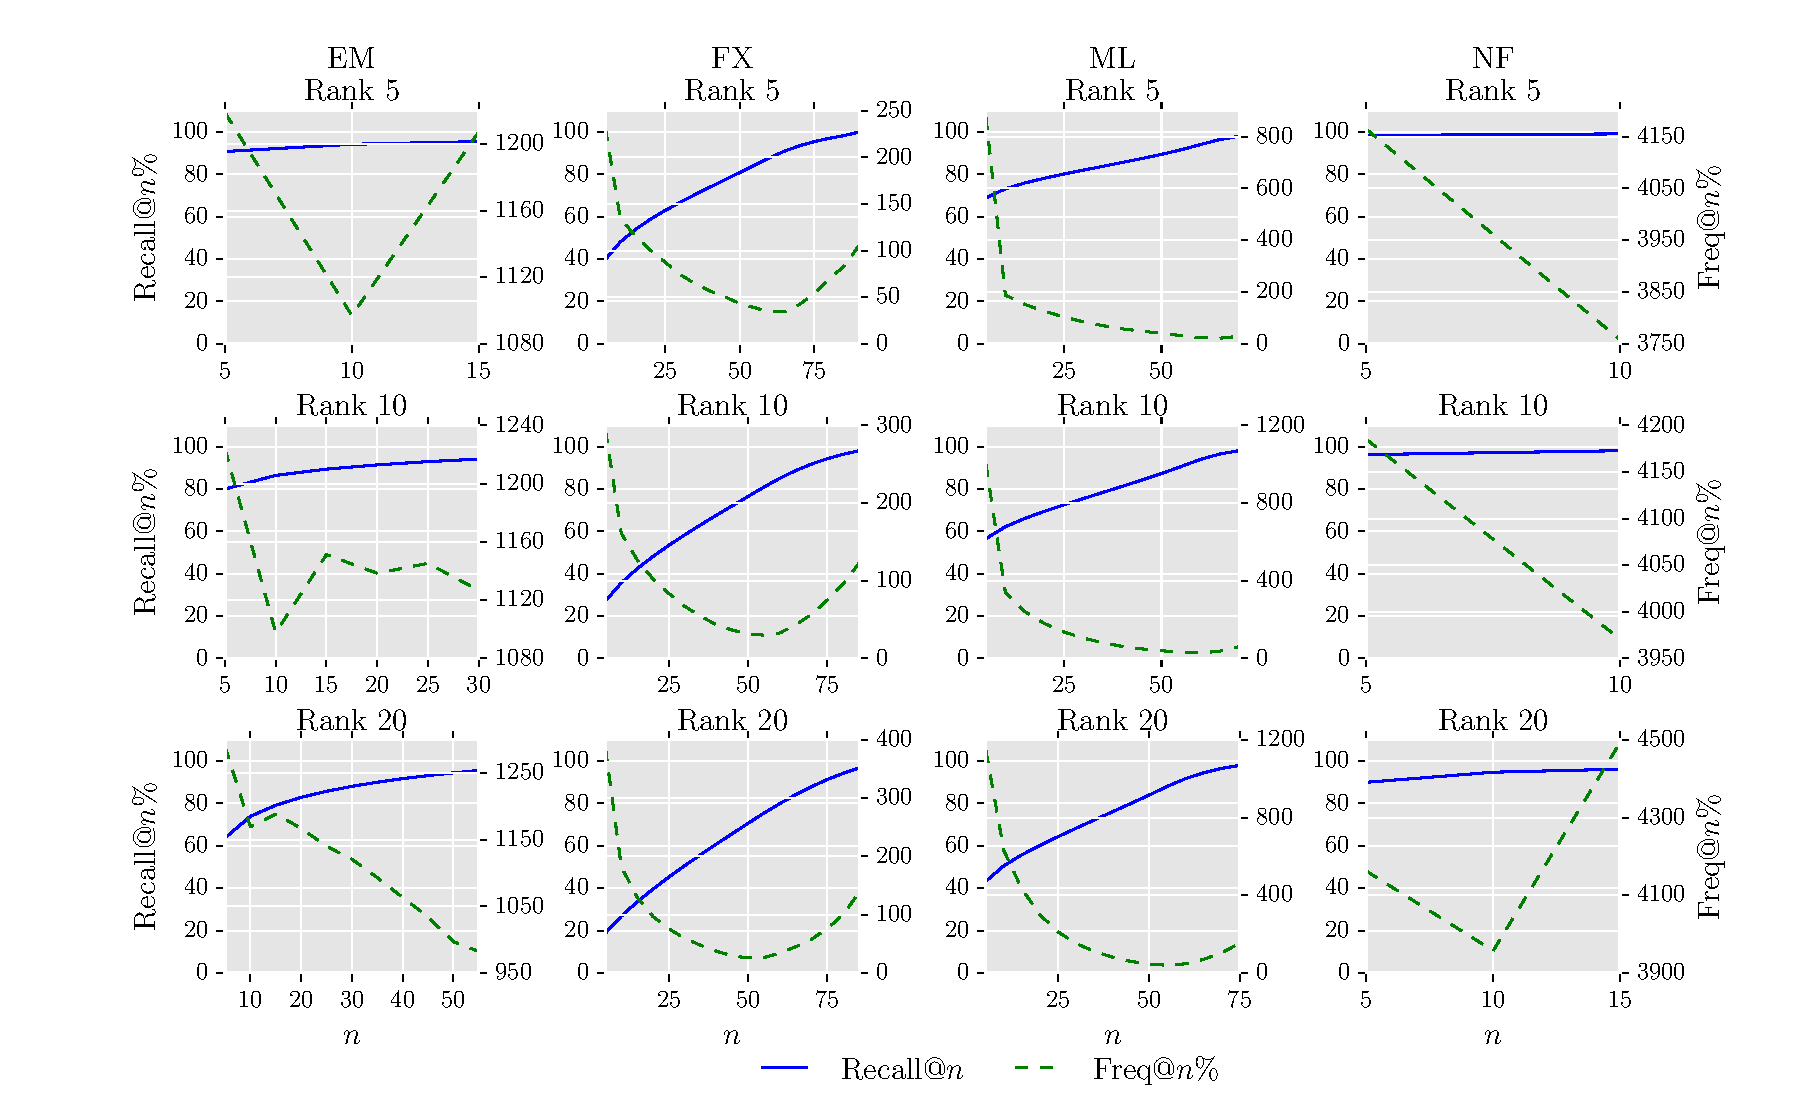
\includegraphics[scale=0.5]{figures/gt_rank_freq} 
  \caption{Recall@$n$\%  and Freq@$n$\% of the \topf of the ground-truth items 
    in ordering by the predictions from the estimated low-rank models.}
  \label{fig:flixmlgtfreq}
\end{figure}

\begin{figure}[bt]
  \hspace*{-1.5cm}
  %\centering
  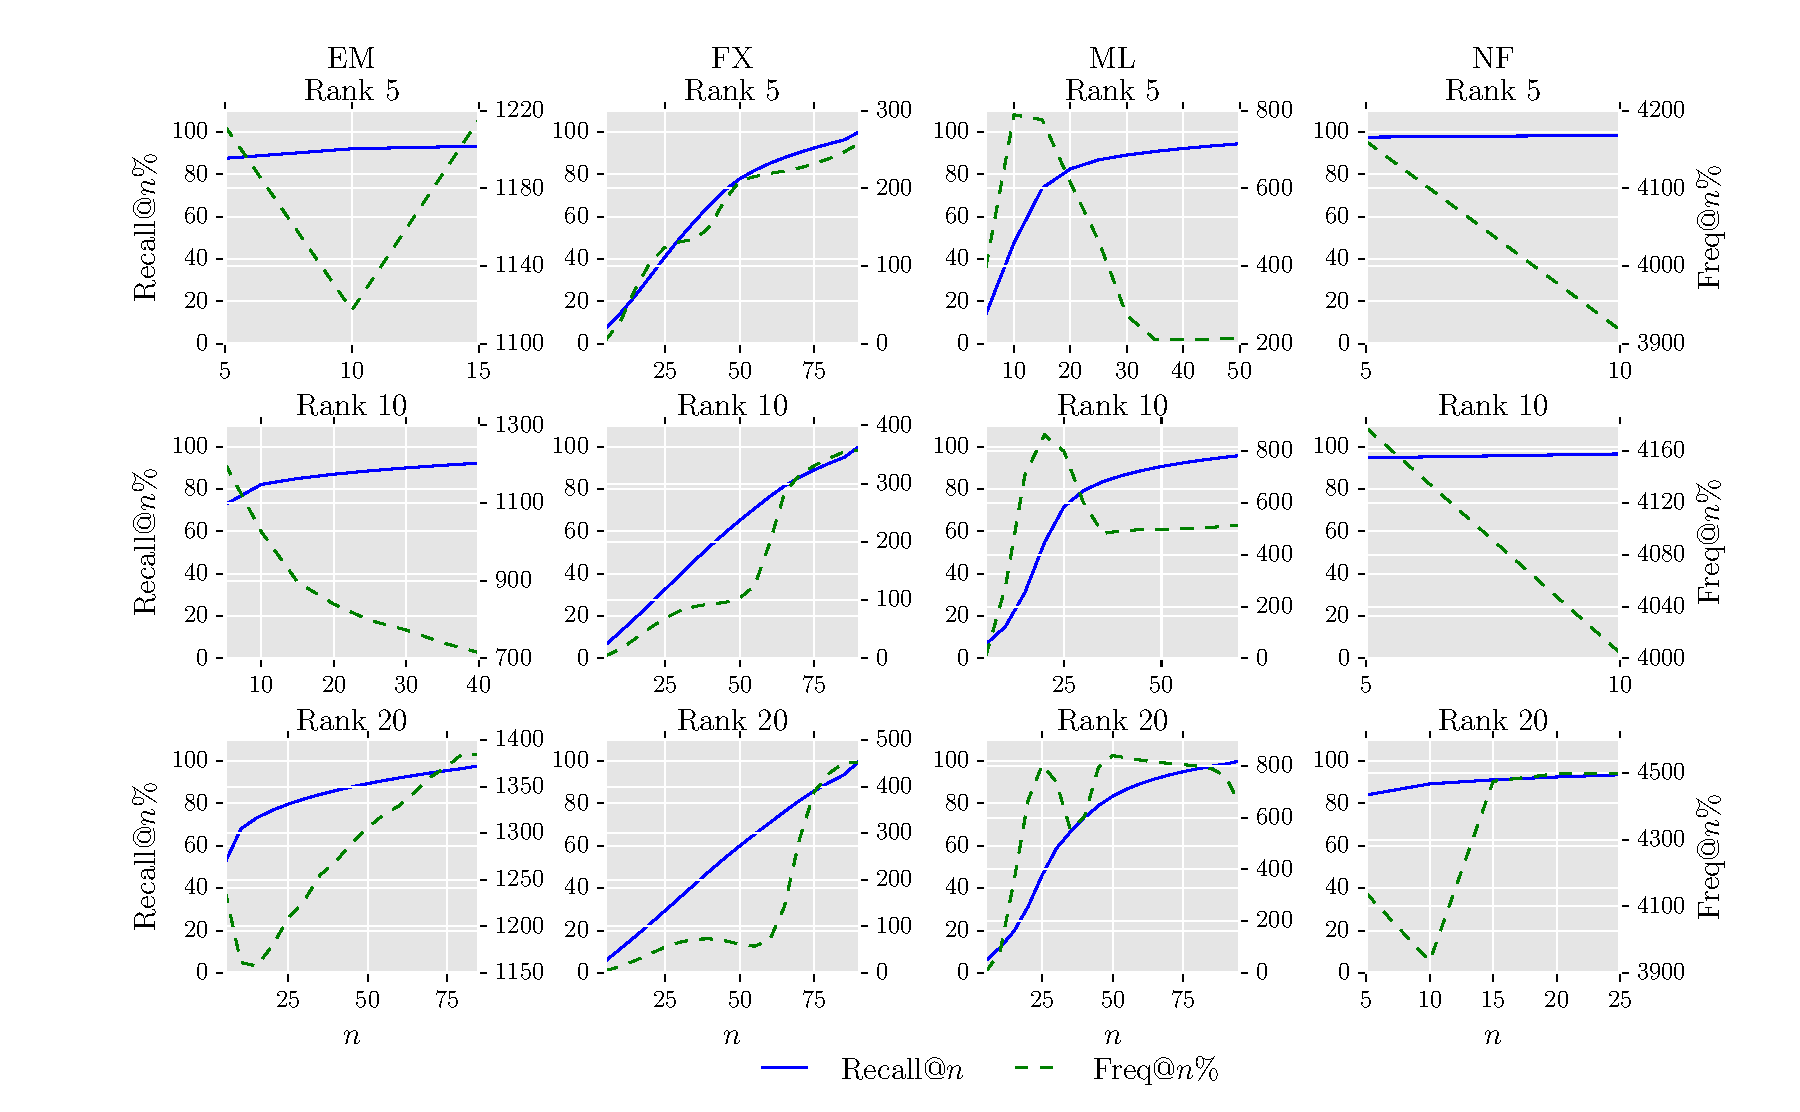
\includegraphics[scale=0.5]{figures/gtLarge_rank_freq} 
  \caption{Recall@$n$\%  and Freq@$n$\% of the \topf of the ground-truth items 
    in ordering by the predictions from the estimated low-rank models initialized with values in the range [0, 5].}
  \label{fig:flixmlgtfreq_Large}
\end{figure}



We investigated how the ranking performance of the estimated low-rank models varies with
the frequency of the items in SYN-REAL matrices.

To this end, for each user we computed the Recall@$n$\% of the items in $G_{u}^{5\%}$, 
i.e., the percentage of the items in $G_{u}^{5\%}$ that are present in
$E_{u}^{n\%}$. Here, $n$ takes the value in [5, 10, 15, ..., 100]. 
Also, we computed the average frequency of the items in
$G_{u}^{5\%}$ that are present in $E_{u}^{n\%}$ but are absent in
$E_{u}^{(n-5)\%}$.  
We will refer to the average frequency of these items as Freq@$n$\%.
As can be seen in Figure~\ref{fig:flixmlgtfreq}, for the datasets with fewer ratings per item, i.e.,
the ML and the FX datasets, the items having low frequency tend to appear
at the end of the ranking. This trend is also seen to some extent in the denser
datasets, i.e., the EM and the NF datasets.
We hypothesize that it is because the low-rank model, i.e., the user and the item latent factors, is
initialized with values close to zero and since items with fewer ratings do not often
occur in the updates during the model estimation they are predicted low
by the estimated low-rank model. 
Therefore, the ranking performance of the estimated low-rank models on SYN-REAL
matrices is not affected by false
positives as both frequent and infrequent items that are rated low will be predicted low
while frequent items that are rated high will be predicted high. 
To test this hypothesis, we initialized the low-rank models with higher values in the
range [0,5] and analyzed the learned models.
Figure~\ref{fig:flixmlgtfreq_Large} shows the Recall@$n\%$ of the items in
$G_{u}^{5\%}$ along with their average frequency, i.e., Freq@$n$\%, for the
estimated low-rank models initialized with higher values.
As can be seen in the figure, unlike the estimated low-rank models
initialized with values close to zero, the items having low frequency does not
necessarily appear in the later buckets.
Additionally, the Recall@$n$ is significantly lower for smaller values of $n$ when
compared with that of the estimated low-rank models initialized with values close to 0. 
This suggests that the model initialization affects both the accuracy and the
ranking performance of the matrix completion-based methods.

\iffalse
We validated this by computing the norm of the singular vectors in users'
latent factors and scaling the corresponding singular vector in items'
latent factors by the computed norm. Next, we examined the items'
frequency and their computed norms from the scaled items' latent
factors. As can be seen in Figure~\ref{fig:em_bx_scatter_norm} for EM and \BX
datasets, the norm of the estimated latent factors
of the infrequent items is comparatively lower than the frequent items, and
hence these items are predicted low by the low-rank models.
\fi

Previously in Section~\ref{ch:matcomp:mf_accu}, we showed that the accuracy of the
estimated low-rank
models is better for items having high frequency.
Considering the analysis of ranking performance, we can reason that the
frequent items that are rated high will be predicted
high by the estimated low-rank model. Hence, the ranking performance of the
estimated low-rank model is 
better for these items than the items that are rated high but are infrequent. 

%-----------------------------------------------------------------------------------------%








